\documentclass[a4paper,12pt]{Latex/Classes/PhDthesisPSnPDF}
\usepackage[utf8]{inputenc}
\usepackage{amsthm}
\usepackage{graphicx}
\usepackage{booktabs}
\usepackage{caption}

% \usepackage[spanish]{babel}
% \input{body/preamble/preamble.Rnw}
% This file contains macros that can be called up from connected TeX files
% It helps to summarise repeated code, e.g. figure insertion (see below).

%%%%%%%%%%%%%%%%%%%%%%%%%%%%%%%%%%%%%%%%%%%%%%
%            Colores de la UNAM              %
%%%%%%%%%%%%%%%%%%%%%%%%%%%%%%%%%%%%%%%%%%%%%%
%Azul Pantone 541  -->(0,63,119) RGB
\definecolor{Azul}{RGB}{128,0,0}

%Oro Pantone 460  -->(234,221,150) RGB
\definecolor{Oro}{RGB}{234,221,150}


%%%%%%%%%%%%%%%%%%%%%%%%%%%%%%%%%%%%%%%%%%%%%%
%            Comandos para líneas            %
%%%%%%%%%%%%%%%%%%%%%%%%%%%%%%%%%%%%%%%%%%%%%%
%Se define un comando \colorvrule para hacer líneas verticales de color con 3 argumentos: color, ancho, alto
\newcommand{\colorvrule}[3]{
\begingroup\color{#1}\vrule width#2 height#3
\endgroup}

%Se define un comando \colorhrule para hacer líneas horizontales de color con 2 argumentos: color, ancho
\newcommand{\colorhrule}[2]{
\begingroup\color{#1}\hrule height#2
\endgroup}

%%%%%%%%%%%%%%%%%%%%%%%%%%%%%%%%%%%%%%%%%%%%%%
%          Comando para derivadas            %
%%%%%%%%%%%%%%%%%%%%%%%%%%%%%%%%%%%%%%%%%%%%%%
\newcommand{\derivada}[3][]{\ensuremath{\dfrac{\mbox{d}^{#1}#2}{\mbox{d}#3^{#1}}}} 
%primer argumento(opcional): orden de la derivada
%segundo argumento: función a derivar
%tercer argumento: variable respecto a la que se deriva


%%%%%%%%%%%%%%%%%%%%%%%%%%%%%%%%%%%%%%%%%%%%%%
%       Comando para la exponencial          %
%%%%%%%%%%%%%%%%%%%%%%%%%%%%%%%%%%%%%%%%%%%%%%
\newcommand{\e}[1][]{\ensuremath{\mbox{e}^{#1}}}
%primer argumento(opcional): exponente de la exponencial




% insert a centered figure with caption and description
% parameters 1:filename, 2:title, 3:description and label
\newcommand{\figuremacro}[3]{
	\begin{figure}[htbp]
		\centering
		\includegraphics[width=1\textwidth]{#1}
		\caption[#2]{\textbf{#2} - #3}
		\label{condicion}
	\end{figure}
}

% insert a centered figure with caption and description AND WIDTH
% parameters 1:filename, 2:title, 3:description and label, 4: textwidth
% textwidth 1 means as text, 0.5 means half the width of the text
\newcommand{\figuremacroW}[4]{
	\begin{figure}[htbp]
		\centering
		\includegraphics[width=#4\textwidth]{#1}
		\caption[#2]{\textbf{#2} - #3}
		\label{#1}
	\end{figure}
}

% inserts a figure with wrapped around text; only suitable for NARROW figs
% o is for outside on a double paged document; others: l, r, i(inside)
% text and figure will each be half of the document width
% note: long captions often crash with adjacent content; take care
% in general: above 2 macro produce more reliable layout
\newcommand{\figuremacroN}[3]{
	\begin{wrapfigure}{o}{0.5\textwidth}
		\centering
		\includegraphics[width=0.48\textwidth]{#1}
		\caption[#2]{{\small\textbf{#2} - #3}}
		\label{#1}
	\end{wrapfigure}
}

% predefined commands by Harish
\newcommand{\PdfPsText}[2]{
  \ifpdf
     #1
  \else
     #2
  \fi
}

\newcommand{\IncludeGraphicsH}[3]{
  \PdfPsText{\includegraphics[height=#2]{#1}}{\includegraphics[bb = #3, height=#2]{#1}}
}

\newcommand{\IncludeGraphicsW}[3]{
  \PdfPsText{\includegraphics[width=#2]{#1}}{\includegraphics[bb = #3, width=#2]{#1}}
}

\newcommand{\InsertFig}[3]{
  \begin{figure}[!htbp]
    \begin{center}
      \leavevmode
      #1
      \caption{#2}
      \label{#3}
    \end{center}
  \end{figure}
}







%%% Local Variables:
%%% mode: latex
%%% TeX-master: "~/Documents/LaTeX/CUEDThesisPSnPDF/thesis"
%%% End:
 
\newtheorem{teorema}{Teorema}
\newtheorem{definicion}{Definición}
% \showboxdepth=5
% \showboxbreadth=5
%%%%%%%%%%%%%%%%%%%%%%%%%%%%%%%%%%%%%%%%%%%%%%%%%%%%%%%%%%%%%%%%%%%%%%%%%%%%%%%%
%                                   DATOS                                      %
%%%%%%%%%%%%%%%%%%%%%%%%%%%%%%%%%%%%%%%%%%%%%%%%%%%%%%%%%%%%%%%%%%%%%%%%%%%%%%%%
\title{Evaluación de la Eficacia de una estrategia de trading basada en Modelo Lineal Generalizado}
\author{Rodrigo Alejandro Serrano Morales} 
\facultad{Facultad de Ciencias Económicas y Sociales\\
Escuela de Estadística y Ciencias Actuariales}                % Nombre de la facultad/escuela
\escudofacultad{images/faces} % Aquí ponen la ruta y nombre del escudo de su facultad, actualmente, la carpeta Latex/Classes/Escudos cuenta con los siguientes escudos:
% "fi_azul" Facultad de ingenieria en color azul
% "fi_negro" Facultad de ingenieria en color negro
% "fc_azul" Facultad de ciencias en color azul
% "fc_negro" Facultad de ciencias en color negro
% Se agradecen sus aportaciones de escudos a jebus.velazquez@gmail.com

\degree{Licenciado en Ciencias Actuariales}        % Carrera
\director{Prof. Jonattan Ramos \& Prof. Eloy Eligon}               % Director de tesis
\degreedate{Marzo 2019}                           % Año de la fecha del examen
\lugar{Caracas}                        % Lugar

%\portadafalse                              % Portada en NEGRO, descomentar y comentar la línea siguiente si se quiere utilizar
\portadatrue                                % Portada en COLOR



%% Opciones del posgrado (descomentar si las necesitan)
	%\posgradotrue                                                    
	%\programa{programa de maestría y doctorado en ingeniería}
	%\campo{Ingeniería Eléctrica - Control}
	%% En caso de que haya comité tutor
	%\comitetrue
	%\ctutoruno{Dr. Emmet L. Brown}
	%\ctutordos{Dr. El Doctor}
%% Datos del jurado                             
	%\presidente{Dr. 1}
	%\secretario{Dr. 2}
	%\vocal{Dr. 3}
	%\supuno{Dr. 4}
	%\supdos{Dr. 5}
	%\institucion{el Instituto de Ingeniería, UNAM}

\keywords{tesis,autor,tutor,etc}            % Palablas clave para los metadatos del PDF
\subject{tema_1,tema_2}                     % Tema para metadatos del PDF  

%%%%%%%%%%%%%%%%%%%%%%%%%%%%%%%%%%%%%%%%%%%%%%%%%%%%%
%                   PORTADA                         %
%%%%%%%%%%%%%%%%%%%%%%%%%%%%%%%%%%%%%%%%%%%%%%%%%%%%%
\usepackage{Sweave}
\begin{document}
\Sconcordance{concordance:main.tex:main.Rnw:%
1 64 1 1 0 14 1}
\Sconcordance{concordance:main.tex:./body/introduccion/introduccion.Rnw:ofs 80:%
1 11 1}
\Sconcordance{concordance:main.tex:./body/chapter1/chapter1.Rnw:ofs 92:%
1 43 1}
\Sconcordance{concordance:main.tex:./body/chapter2/chapter2.Rnw:ofs 136:%
1 255 1 1 18 1 2 17 1}
\Sconcordance{concordance:main.tex:./body/chapter3/chapter3.Rnw:ofs 411:%
1 95 1 1 64 3 1 2 2 32 1}
\Sconcordance{concordance:main.tex:./body/chapter4/chapter4.Rnw:ofs 545:%
1 15 1 1 14 3 1 2 2 13 1 1 8 1 3 7 1 1 8 1 2 4 1 1 74 2 1 1 3 1 2 8 1 1 %
3 1 2 8 1 1 3 1 2 8 1 1 12 5 1 1 9 1 2 12 1 1 14 1 2 9 1 1 3 1 2 13 1 1 %
7 1 2 4 1 1 7 3 1 1 7 1 2 22 1 1 3 9 0 1 2 1 1 1 32 1 2 8 0 1 1 7 0 1 2 %
9 0 1 1 10 0 1 2 12 1 1 7 12 0 1 2 3 1 1 6 12 0 1 2 3 1 1 6 12 0 1 2 4 %
1 1 6 12 0 1 2 3 1 1 6 12 0 1 2 4 1 1 6 12 0 1 2 7 1 1 37 2 1 1 2 15 0 %
1 2 3 1 1 26 5 1 1 9 1 2 4 1 1 24 3 1 1 9 1 2 15 1 1 17 2 1 1 2 14 0 1 %
2 3 1 1 27 2 1 1 2 11 0 1 2 2 1}
\Sconcordance{concordance:main.tex:./body/conclusion/conclusion.Rnw:ofs 976:%
1 7 1 1 20 3 1 1 6 1 2 15 1}
\Sconcordance{concordance:main.tex:./body/anexos/anexos.Rnw:ofs 1005:%
1 9 1 1 2 12 0 1 2 3 1 1 2 12 0 1 2 2 1 1 2 12 0 1 2 5 1 1 2 12 0 1 2 3 %
1 1 2 12 0 1 2 2 1 1 2 12 0 1 2 6 1 1 2 12 0 1 2 3 1 1 2 12 0 1 2 3 1 1 %
2 12 0 1 2 5 1 1 2 12 0 1 2 3 1 1 2 12 0 1 2 2 1 1 2 12 0 1 2 6 1 1 2 %
12 0 1 2 3 1 1 2 12 0 1 2 2 1 1 2 12 0 1 2 5 1 1 2 12 0 1 2 3 1 1 2 12 %
0 1 2 2 1 1 2 12 0 1 2 6 1 1 2 12 0 1 2 4 1 1 2 12 0 1 2 2 1 1 2 12 0 1 %
2 5 1 1 2 12 0 1 2 3 1 1 2 12 0 1 2 2 1 1 2 12 0 1 2 1 1}
\Sconcordance{concordance:main.tex:./body/bibliografia/bibliografia.Rnw:ofs 1432:%
1 37 1}
\Sconcordance{concordance:main.tex:main.Rnw:ofs 1470:%
88 1 1}


\maketitle									% Se redefinió este comando en el archivo de la clase para generar automáticamente la portada a partir de los datos

\newpage\renewcommand{\thepage}{\arabic{page}}\setcounter{page}{1} 

% !TeX root = ./main.Rnw
%\SweaveUTF8

\begin{dedication}
Dedicado a mis padres y a mi hermana, por ser los pilares de mi vida y ser mi motivo de haber cumplido esta meta.
\end{dedication}
% !TeX root = ./main.Rnw
%\SweaveUTF8
\newpage
\chapter*{Agradecimientos}

Agradecimientos




  \begin{flushright}
  \textbf{Gracias}
  \end{flushright}

\tableofcontents
\listoffigures
\listoftables


% !TeX root = ./main.Rnw
%\SweaveUTF8

\chapter*{Introducción}
\addcontentsline{toc}{chapter}{Introduccion}

Las economías de países latinoamericanos son reconocidas históricamente por depender en gran magnitud del comercio de sus materias primas, lo cual hace que el comercio con dichos commodities resulte de gran impacto para el gasto fiscal y para la balanza de pagos, esto deja como consecuencia, la necesidad de los actores económicos de estudiar el riesgo a profundidad para poder evitar resultados que reduzcan sus retornos positivos.\\ 

% \SweaveInput{body/chapter1/chapter1.Rnw}
% \SweaveInput{body/chapter2/chapter2.Rnw}
% !TeX root = ./main.Rnw
%\SweaveUTF8

\chapter{Marco Metódico}
\section{Análisis Exploratorio de los datos}

\subsection{Datos OHLC y Fuente de los datos}

La estructura de los datos utilizados en el trabajo es de tipo OHLC por sus siglas en inglés Open, High, Low, Close. La misma, resume en 4 registros el comportamiento del precio del activo (Apertura, Cierre, Mínimo y Máximo) en un intervalo de tiempo. En el caso de la presente investigación, de un día. Este tipo de dato provee la información necesaria para cubrir las exigencia del modelo, tanto para la creación de la variable dependiente como para el cálculo de los indicadores técnicos. 

Los datos fueron extraídos del portal www.investing.com, uno de los portales financieros con mayor prestigio en el mundo. Fue fundado en 2007 y es conocido por su prestigioso calendario económico y directorio de brokers.

\subsection{Series de Índices}

El universo de estudio está representado por los índices bursátiles de los mercados financieros existentes entre el período 26/10/2008 - 18/01/2019. Un índice búrsatil es un promedio de los precios de los activos que representan un mercado o sector determinado. Los mismos sirven como 'benchmark' o referencia de la economía de un país, sector financiero, etc. En el ámbito de los 'hedge funds' son una referencia para medir la rentabilidad de una estrategia de inversión y el riesgo del mercado.

En la presente investigación se utilizan los índices como reflejo del comportamiento de varios activos, de esta manera, se mide la estrategia en un sector y no en un instrumeto en específico. Otras de las ventajas de utilizar los índices es que al representar un promedio de varios activos, sus variaciones son menos drásticas. La muestra está constituida por 5 índices bursátiles que representan distintos mercados del mundo: NASDAQ, NIKKEI, FTSE 100, BOVESPA y SP500.

% hablar de cada indice


\begin{figure}[H]
\setkeys{Gin}{width =0.8\textwidth}
\centering
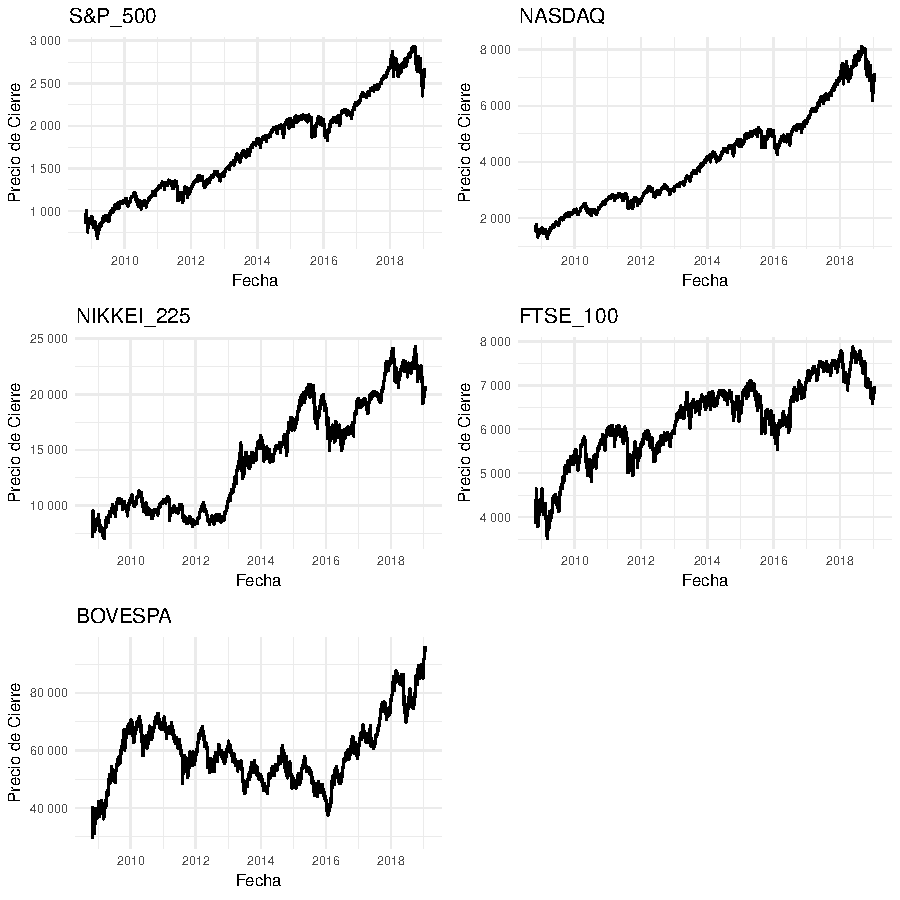
\includegraphics{main-002}
\caption{Precios de Cierre de los índices en el período de estudio (26/10/2008 - 18/01/2019)}
\end{figure}

\section{Entrenamiento del Modelo}

\subsection{Variable dependiente}

Las decisiones de entrada en el trading pueden ser producto de muchos factores, en la presente investigación se analiza el enfoque donde se define un porcentaje objetivo de ganancia y se intenta predecir si dicho objetivo se materializará en un futuro cercano, sin que se haya concretado una venta por Stop Loss. Este enfoque reduce la toma de decisión en una variable tal que:

$$
P_{X}(x) = 
\begin{array}{ll} 
\ \ \ \ p \ ; \qquad x = c
\\
\ 1-p \ ; \qquad x = -d
\end{array}
$$

Dado los datos OHLC del activo es posible identificar los períodos en donde se materializa la variable dependiente. la identificación se realiza, comparando el precio de cierre con los precios máximos y mínimos de las siguientes h observaciones, donde h es el número de períodos, en este caso días en los cuales se desea evaluar la condición.

En la práctica se identifica los registros que cumplen con esta condición añadiendo una columna a la data donde incluimos 'buy' para identificar los registros donde se da la señal y 'stay' en caso de que no haya ocurrido o hubiese ocurrido primero el retroceso del precio.

\subsection{Indicadores Técnicos como variables predictoras}

Los indicadores a utilizar fueron seleccionados buscando recoger la mayor información posible sobre el precio del activo, se pueden resumir en tres categorías: tendencia, momentum y volatilidad.

No es de interés en la presente investigación describir como funciona cada indicador para la toma de decisiones en el trading basado en fundamentos técnicos. Cada indicador puede utilizarse de distintas maneras, calcularse con distintos parámetros y asociarse a discreción del trader, lo que conlleva a un sin fin de reglas de asciación. 

Lo que busca la investigación es utilizar la relación entre estos indicadores como variables independientes que ayuden al modelo a predecir oportunidades de entradas. En este sentido se asume la existencia de una dinámica local del mercado que puede ser predecida con ayuda de estos indicadores.

A continuación se presentan los indicadores utilizados:

\begin{itemize}
\item Retornos con respecto al precio de Cierre.
\item RSI (Relative Strength Index) de 14 períodos, el cual es un indicador de volatilidad.
\item MACD (Moving Average Converge/Divergence) el cual es una diferencia de dos EMAs (Exponential Moving Average) de 12 y 26 períodos. Este es un indicador de tendencia que se complementa con un MA(Moving Averge) de 9 períodos. 
\item ADX (Average Directional Index), este es un indicador que utiliza dos indicadores de dirección +Di y -Di, se calculó en base a 14 períodos y mide tendencia.
\item Bandas de Bollinger, el cual es un indicador de tendencia y volatilidad, utiliza dos bandas calculadas a partir de una media movil con desviaciones estándar. Se utilizó en base a 14 períodos y una desviación de 2.5.
\item ATR (Average True Range), es un indicador de volatilidad calculado a partir de los máximos y mínimos de un período, en este caso 14.
\end{itemize}

Estos indicadores están fuertemente correlacionados por lo que se decidió, disminuir el numero de variables dejando solo las más representativas de cada indicador.

\begin{figure}[H]
\setkeys{Gin}{width = 0.6\textwidth}
\centering
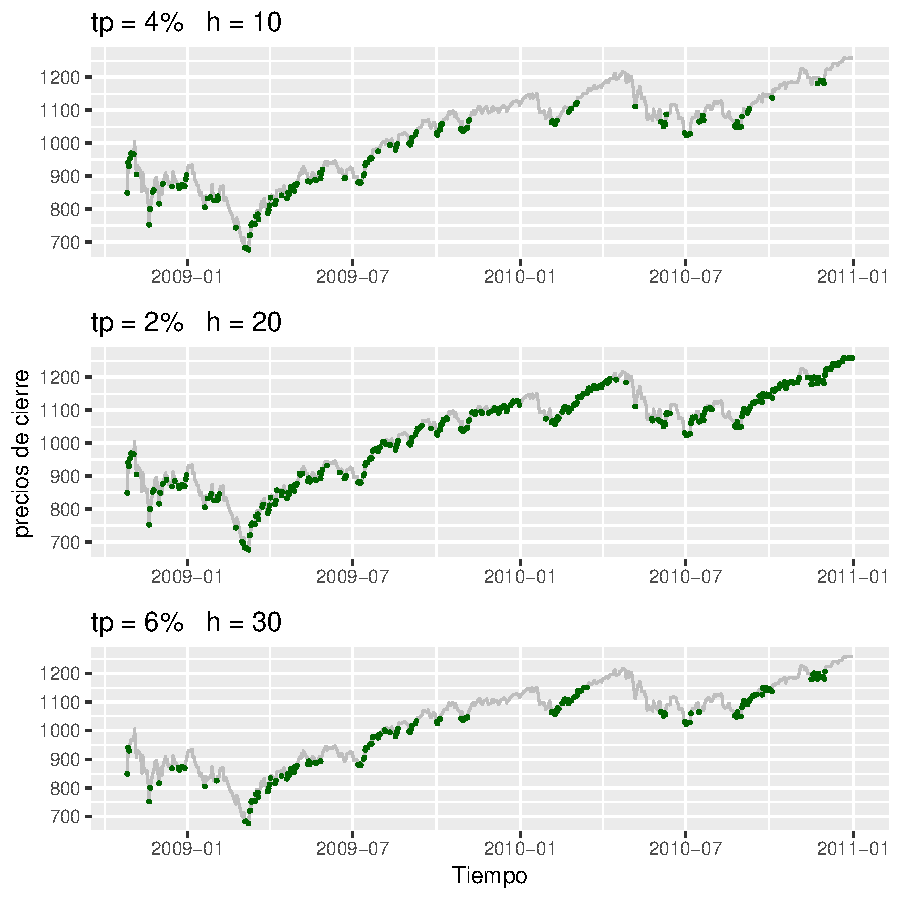
\includegraphics{main-003}
\caption{Correlación entre indicadores originales calculados con los precios del S&P500 en el primer período de entrenamiento(01/01/2009 - 31/12/2012)}
\end{figure}

Como se puede observar existe alta correlación entre las distintas variables del precio (Apertura, Cierre, Máximo y Mínimo) por lo que se decidió trabajar solo con los precios de cierre dado que ésta es la misma utilizada para determinar la variable dependiente. Así mismo se observa alta correlación entre los rezagos de los rendimientos, para esto se decidió trabajar solo con los rezagos de 1, 3 y 5 períodos. Por su parte se descarta la variable dip -elemento utilizado en el indicador ADX- por su fuerte correlación con el RSI. Se determina lo mismo para la banda inferior del indicador de Bollinger.

En la figura -- se muestra las correlaciones de las variables definitivas

\begin{figure}[H]
\setkeys{Gin}{width = 0.6\textwidth}
\centering
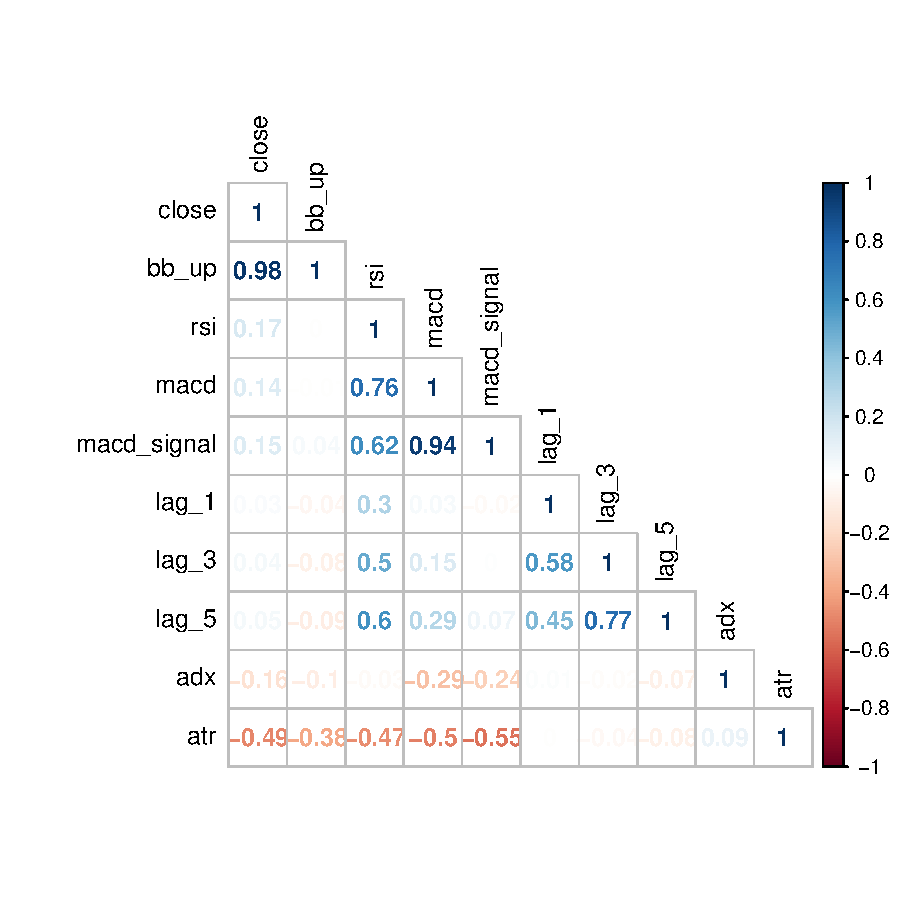
\includegraphics{main-004}
\caption{Correlación entre indicadores definitivos calculados con los precios del S&P500 en el primer período de entrenamiento(01/01/2009 - 31/12/2012)}
\end{figure}

Ahora bien, la idea base de la investigación era utilizar los valores de cada indicador como variables predictora. Dado que el cálculo de todos los indicadores provienen de la misma variable -precio del activo, en la mayoría de los casos precio de cierre-, exite una alta colinealidad entre ellos, la idea de utilizar el ACP es precisamente para enfrentar este problema como se detallará más adelante. Sin embargo, es de notar que los valores de los indicadores por sí solos no proveen un poder predictivo, lo que realmente usa el trader son las asociaciones entre indicadores para encontrar patrones. 

Se decidió entonces, utilizar como predictores no los indicadores por si solos, sino, las relaciones entre cada uno de ellos. Esto se abordo agregando al modelo las interacciones entre todos los indicador, y removiendo los valores de los indicadores por sí solos. De esta manera el hecho de utilizar ACP, no solo es visto ahora como una manera de remover la colinealidad entre predictores sino como método de reducción de variables, ya que el modelo pasó de tener 10 predictores -incluyendo el precio de cierre- a 45.

A continuación se presentan una serie de gráficos para reflejar lo anteriormente expuesto en relación a la colinealidad entre los indicadores.





\subsection{Validación Cruzada en Series de Tiempo}

La validación Cruzada es un metódo de validación y prueba que consiste en dividir los registros aleatoriamente en grupos de similar tamaño. El primer grupo es utilizado como validación del modelo que ha sido entrenado en el resto de los datos, este proceso se realiza k veces, y el resultado final es el promedio arrojado por cada una de las k validaciones.

Ahora bien este método asume que no existe relación entre las observaciones, es decir que son independientes. Esto no es verdad en el caso de las series de tiempo debido a la condicion de autoregresión. Por lo tanto al dividir la data se debe respetar el orden temporal de cada observación. 

\subsection{WalkForward Backtesting}

Al principio de la investigación se implementó el método de entrenamiento, validación y prueba comúnmente utilizado, en donde la mayor parte de la data es destinada a entrenamiento del modelo, otra seccion es destinada a validación, para elegir los parámetros óptimos, y finalmente se testeaba el modelo en la data de prueba. Sin embargo este tipo de metodología en opinión del investigador no es el más óptimo para desarrollar el presente modelo, dado el dinamísmo de los mercados bursátiles la estrategia no puede permanecer estática en el tiempo.

Para contrarestar esta situación se opto por el método de $backtesting Walkforward$, el cual consiste en entrenar el modelo en un período base de data, en este caso los primeros 4 años de estudio, posteriormente se aplica la estrategia en el año siguiente y se obtiene los primeros resultados. Luego este año de aplicación es incluído en la data de entrenamiento -es decir, la data de entrenamiento pasa a ser de 5 años- y se evalúa el modelo en el siguiente año. De esta manera, contemplamos el dinamísmo del mercado permitiendole al modelo -y por ende a la estrategia- utilizar el período mas reciente con respecto al cual será implementado. En la presente figura se ilustra la metodología implementada.

\begin{figure}[ht]
\begin{center}
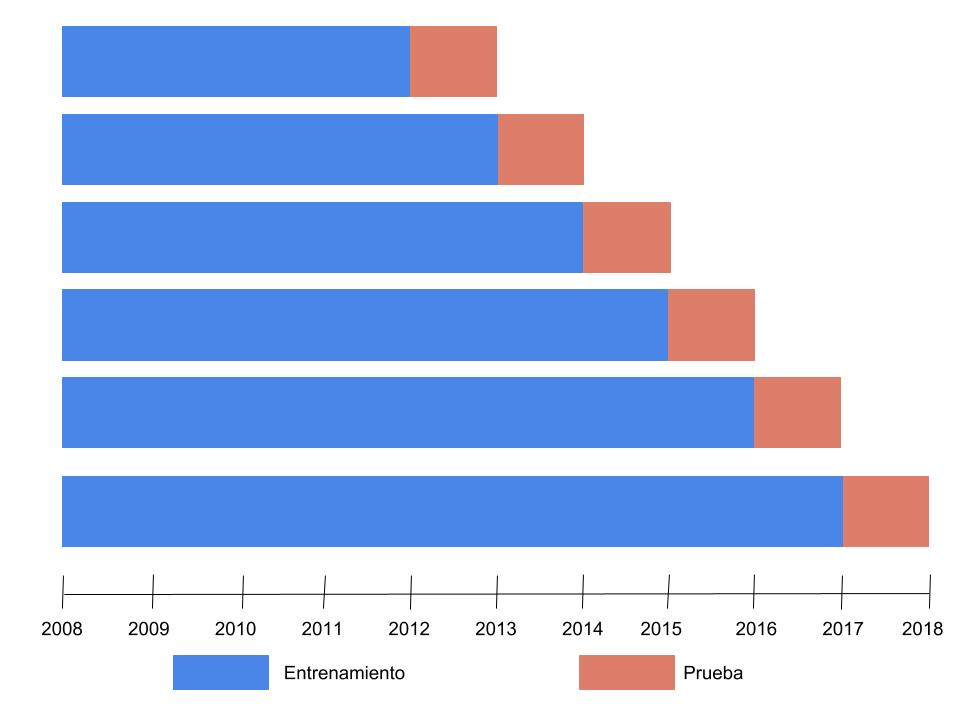
\includegraphics[width=2.5in]{images/walkforward_plot}
\end{center}
\caption{Metodología WalkForward}
\end{figure}

Otra de las caracteristicas de la metodología que se modificó fue la elección de los parámetros óptimos. Previamente se utilizaba la data de validación para buscar la combinación de parámetros óptima. Ahora bien en la metodología de Walkforward se utilizan los mismo parámetros. A opinión del investigador al buscar los mejores parámetros se estaría incurriendo en un posible cesgo de sobreoptimización. El hecho de que en un año determinado unas configuraciones óptimas den los mejores resultados no asegura que se replique en el siguiente año.

La selección de los parámetros debería ser un estudio previo de la serie financiera a testear. Evidentemente al seleccionar un período de tiempo mas corto se obtendrán menos observaciones que cumplan con el patrón por lo tanto se estaría en presencia de un problema de data imbalanceada que debe tener un tratamiento distinto. Por otro lado el utilizar un horizonte mayor no representa gran cambio en el número de ocurrencias, pero sí en el caso de que la transacción quede abierta -hay recordar que h representa una condición de salida para la estrategia de no ocurrir el target ni el stop loss-. La estrategia implementada en la invstigación toma un horizonte de 20 períodos ya que este valor representa un umbral para la ocurrencia del objetivo.


\begin{figure}[H]
\setkeys{Gin}{width = 0.8\textwidth}
\centering
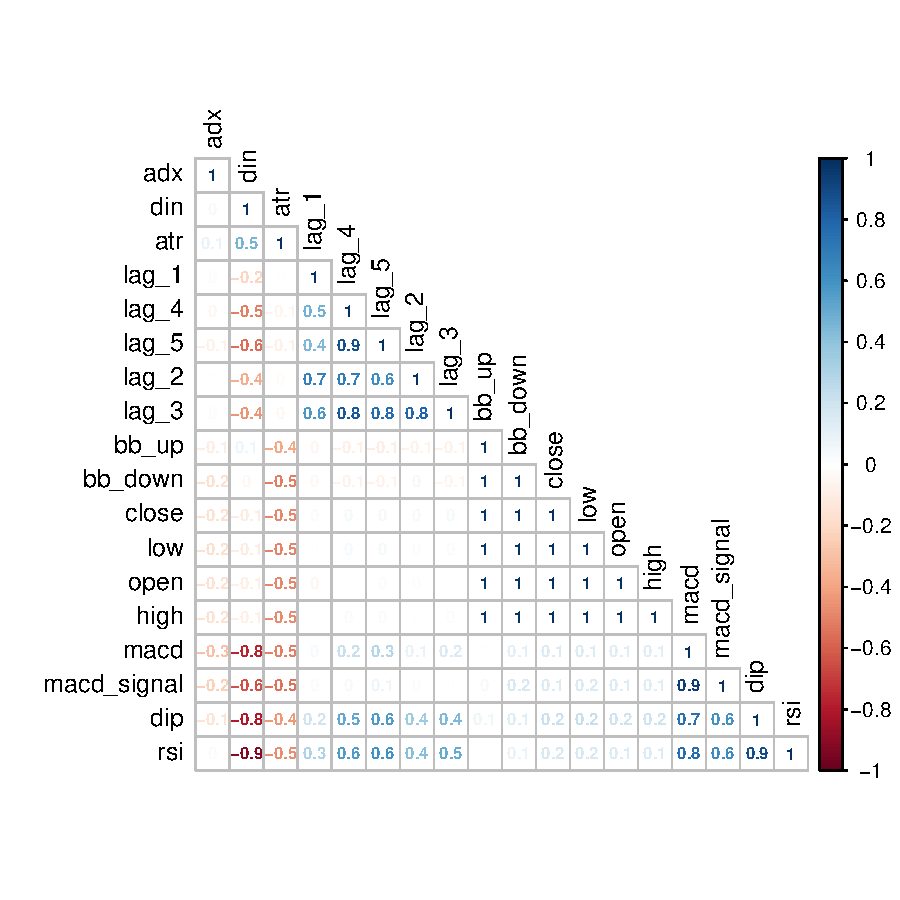
\includegraphics{main-006}
\caption{Observaciones que presentan ocurrencias con sl = 2.5\%, en el primer conjunto de datos de entrenamiento (26/10/2008 - 31/12/2010) para el índice S&P500, para diferentes valores de tp y h}
\end{figure}

\subsection{Reducción de la dimensión con Análisis de Componentes Principales}

La técnica que utiliza el ánalisis de componentes principales (PCA) para reducir el numero de variables predictoras es conocido como Principal Component Regression (PCR). PCR es utilizado para extraer la información más importante de una matríz de datos multivariante y expresar ésta información en nuevas variables llamadas componentes principales. Éstas son una combinación lineal de las variables originales. Aunque el número de componentes principañes puede ser igual al número de variables, la idea es utilizar un grupo reducido de componentes que maximizen la variación.

Por su parte el modelo propuesto utiliza las interacciones entre las variables predictoras, esto aumenta el número de variables de 10 a 45, las cuales además en muchos casos están correlacionadas. Al utilizar PCR se reduce el número de variables en la mayoría de los casos a 7 componentes donde las dos primeras contienen al rededor del 25\% de la variación, es importante recordar que esta reducción se realiza en cada período de entrenamiento. 

A continuación se analizan los resultados de los componentes arrojados por el modelo en el primer período de entrenamiento (2009-2012) utilizando el índice S&P500, en esta sección se referira a ésta como 'matriz de datos'.


Los eigenvalores miden la cantidad de variación retenida por cada componente. Los eigenvalores son mayores para los primeros componentes, dado que el primer componente busca maximizar la cantidad de variación de la matriz de datos, por lo que cada vez es menor la cantidad de variación retenida por cada componente.

Los eigenvalores pueden usarse para establecer el número de componentes a utilizar. Para el modelo se estableció que en cada período de entrenamiento se utilizaría la cantidad de componentes necesarias para explicar el 85\% de la variación de la matríz de datos.

La proporción de variación explicada por cada eigenvalor viene dada de dividir cada eigenvalor por su sumatoria, en este caso 45 -el número de variables originales-.

Un eigenvalor mayor que 1 indica que el componente tiene mayor variación que la contenida en una de las variables originales. En la figura -- Se puede observar que el 85\% de la variación esta contenida en los primeros 7 componentes. Igualmente se aprecia que el eigenvalor de los 10 PCs es mayor que 1. 

\begin{figure}[H]
\setkeys{Gin}{width = 0.8\textwidth}
\centering
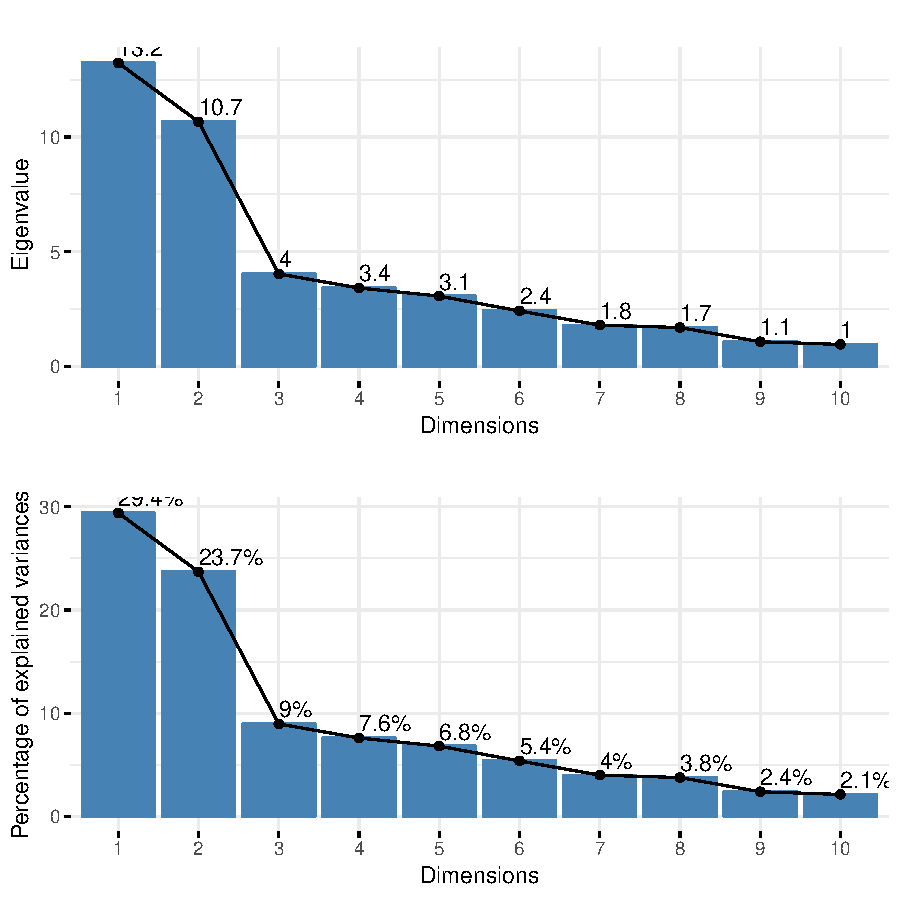
\includegraphics{main-008}
\caption{Eigenvalores y Porcentaje de contribución para los 10 componentes más importantes obtenidos por la matríz de datos}
\end{figure}

La contribución de las variables representan la variabilidad contenida en un componente. Las variables correlacionadas con el componente principal 1 (PC1) y PC2 son las más importantes en explicar la variabilidad en la matráz de datos. Aquellas que no se correlacionan con ninguna componente son desechadas por su baja contribución. En la figura -- se observa la contribución de las primeras 30 variables en PC1, PC2 y la contribución obtenida en ambas.

\begin{figure}[H]
\setkeys{Gin}{width = 0.8\textwidth}
\centering
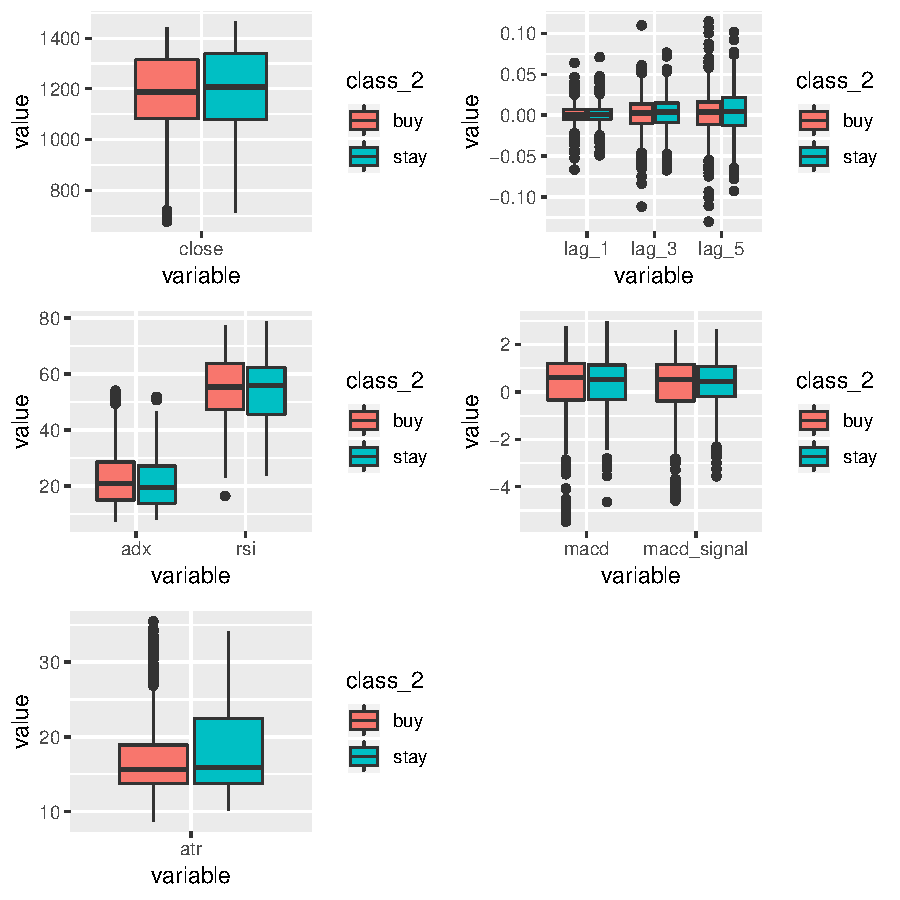
\includegraphics{main-009}
\caption{Contribución de cada variable para PC1, PC2 y el total de la contribución en ambos componentes}
\end{figure}

La línea roja indica el promedio esperado de contribución si las variables fueran uniformes, es decir $ \frac{1}{N° de Variables} = \frac{1}{45} = 2,2\%$. Una variable sobre este umbral se considera importante en la contribución al componente. Se aprecia como las interacciones que predominan en ambos componentes estan relacionadas con el indicador MACD.

La calidad de representación en el gráfico viene dada por el valor de $Cos^2$, el cual se refiere a la importancia que tiene la variable para interpretar el componente. Para una variable la suma de $Cos^2$ en todas las componentes equivale a 1. En la figura -- se muestra los valores de $Cos^2$ para las primeras 2 componentes

\begin{figure}[H]
\setkeys{Gin}{width = 0.8\textwidth}
\centering
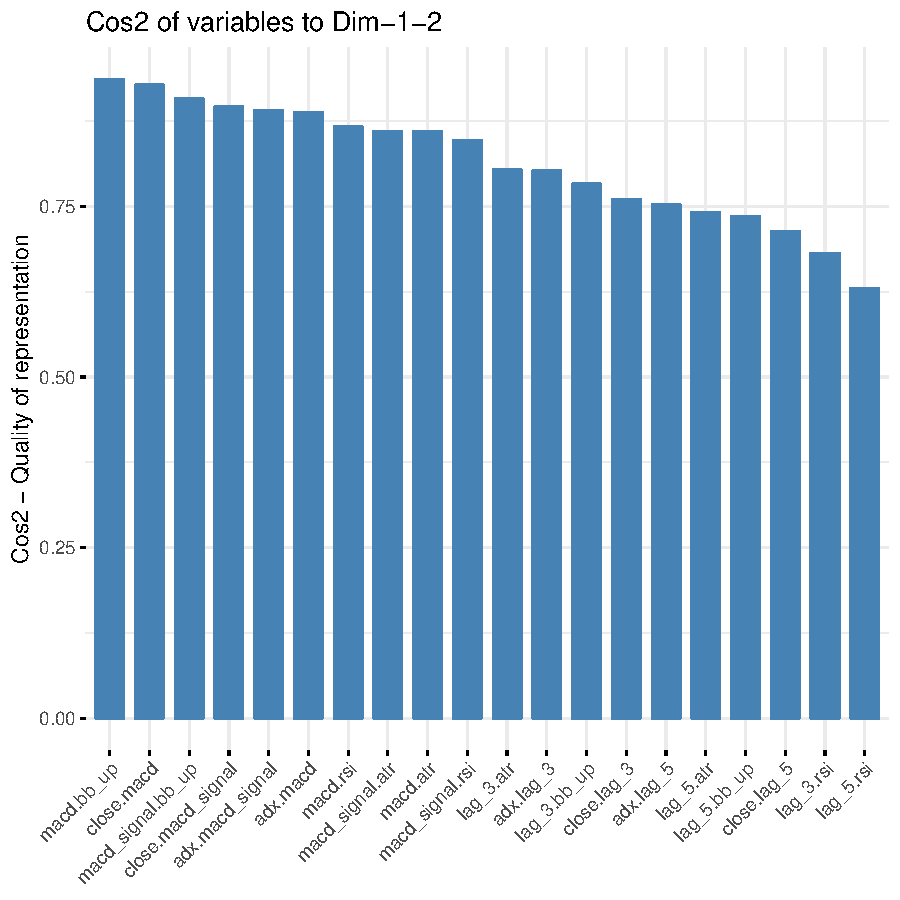
\includegraphics{main-010}
\caption{Calidad de representación medida por $Cos^2$ de cada variable en PC1 y PC2}
\end{figure}

El gráfico de correlación ó Factor map muestra la relación entre las variables. Las claves para su interpretación son:

\begin{itemize}
\item Las variables positivamente correlacionadas se encuentran agrupadas
\item Las variables negativamente correlacionadas se posicionan en quadrantes opuestos, es decir en lados contrarios.
\item La distancia entre las variables y el origen mide la calidad de representación de las variables en el gráfico. Mientras más alejado del origen, mejor representadas 
\end{itemize}

En la figura -- se observa el gráfico de correlación para PC1 y PC2, el color de cada variable viene dado por su contribución, mientras mas oscuro menor es su contribución a los componentes.

\begin{figure}[H]
\setkeys{Gin}{width = 0.8\textwidth}
\centering
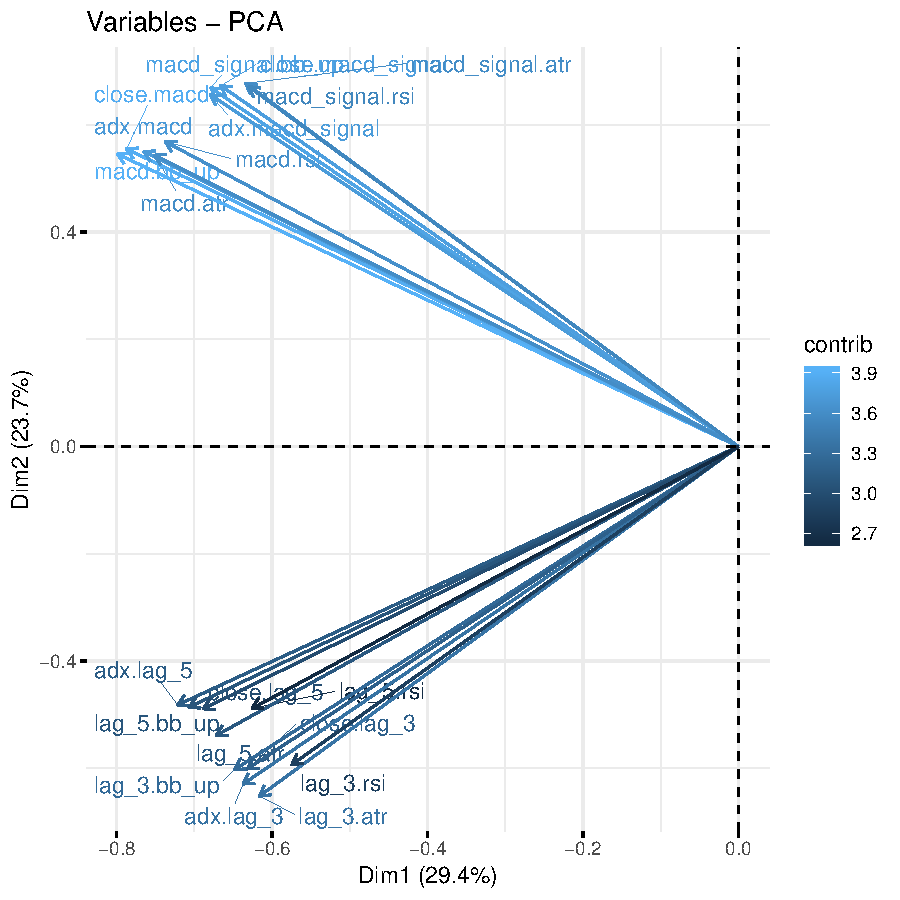
\includegraphics{main-011}
\caption{Gráfico de Correlación entre PC1 y PC2}
\end{figure}

% !TeX root = ./main.Rnw
%\SweaveUTF8

\chapter{Análisis de Resultados}

En el presente capítulo se realiza la descripción de los resultados obtenidos despues de la aplicación del método propuesto para la estrategia. De igual modo, se presentan los resultados arrojados por las pruebas de Backtesting simulando las entradas y salidas.

\section{Series de Rendimientos}







\begin{center}
\captionof{table}[Resultados]{\textbf{Resultados}}
\begin{minipage}{.45\textwidth}
% latex table generated in R 3.5.2 by xtable 1.8-3 package
% Wed Feb  6 18:44:33 2019
\begin{table}[ht]
\centering
\begin{tabular}{rrrrr}
  \hline
 & Estimate & Std. Error & z value & Pr($>$$|$z$|$) \\ 
  \hline
(Intercept) & -0.3599 & 0.0645 & -5.58 & 0.0000 \\ 
  PC1 & -0.0146 & 0.0181 & -0.81 & 0.4183 \\ 
  PC2 & -0.0134 & 0.0203 & -0.66 & 0.5085 \\ 
  PC3 & 0.0050 & 0.0327 & 0.15 & 0.8779 \\ 
  PC4 & 0.0873 & 0.0353 & 2.47 & 0.0135 \\ 
  PC5 & -0.0222 & 0.0373 & -0.60 & 0.5514 \\ 
  PC6 & -0.0158 & 0.0425 & -0.37 & 0.7100 \\ 
  PC7 & 0.1057 & 0.0484 & 2.18 & 0.0289 \\ 
   \hline
\end{tabular}
\end{table}\captionof*{table}{Fuente: Cálculos propios}
\end{center}
\end{minipage}

\begin{minipage}{.45\textwidth}
\begin{center}
% latex table generated in R 3.5.2 by xtable 1.8-3 package
% Wed Feb  6 18:44:33 2019
\begin{table}[ht]
\centering
\begin{tabular}{rrrrr}
  \hline
 & Estimate & Std. Error & z value & Pr($>$$|$z$|$) \\ 
  \hline
(Intercept) & -0.4093 & 0.0580 & -7.06 & 0.0000 \\ 
  PC1 & 0.0222 & 0.0165 & 1.35 & 0.1785 \\ 
  PC2 & -0.0072 & 0.0182 & -0.40 & 0.6925 \\ 
  PC3 & 0.0169 & 0.0290 & 0.58 & 0.5596 \\ 
  PC4 & 0.0537 & 0.0307 & 1.75 & 0.0800 \\ 
  PC5 & 0.0237 & 0.0336 & 0.71 & 0.4797 \\ 
  PC6 & 0.0393 & 0.0365 & 1.08 & 0.2817 \\ 
  PC7 & -0.1222 & 0.0414 & -2.95 & 0.0032 \\ 
   \hline
\end{tabular}
\end{table}\captionof*{table}{Fuente: Cálculods propios}
\end{center}
\end{minipage}

% \begin{center}
% \captionof{table}[Resultados]{\textbf{Resultados}}
% <<echo=FALSE, results=tex>>=
% library(xtable)
% a <- xtable(summary(list_model[[1]][[1]]))
% a
% @
% \captionof*{table}{Fuente: Cálculos propios}
% \end{center}

% \begin{center}
% \captionof{table}[Resultados del contraste Ljung-Box]{\textbf{Resultados del contraste Ljung-Box}}
% <<echo=FALSE, results=tex>>=
% lj_petroleo <- Box.test(return_petroleo^2, lag = 10, type = 'Ljung-Box')
% lj_harinasoja <- Box.test(return_harinasoja^2, lag = 10, type = 'Ljung-Box')
% lj_oro <- Box.test(return_oro^2, lag = 10, type = 'Ljung-Box')
% lj_aluminio <- Box.test(return_aluminio^2, lag = 10, type = 'Ljung-Box')
% lj_cacao <- Box.test(return_cacao^2, lag = 10, type = 'Ljung-Box')
% boxtable<-data.frame(c(lj_petroleo$statistic,lj_petroleo$p.value),c(lj_harinasoja$statistic,lj_harinasoja$p.value),
% c(lj_oro$statistic,lj_oro$p.value),c(lj_aluminio$statistic,lj_aluminio$p.value),c(lj_cacao$statistic,lj_cacao$p.value))
% rownames(boxtable)<-c("Estadístico de Contraste","P-value")
% colnames(boxtable)<-c("Petróleo","Harina de Soja","Oro","Aluminio","Cacao")
% xtable(boxtable,digits=4)
% @
% \captionof*{table}{Fuente: Cálculos propios}
% \end{center}

% !TeX root = ./main.Rnw
%\SweaveUTF8

\chapter*{Conclusiones y Recomendaciones}
\addcontentsline{toc}{chapter}{Conclusiones y Recomendaciones}



% !TeX root = ./main.Rnw
%\SweaveUTF8

\chapter*{Lista de Referencias}
\addcontentsline{toc}{chapter}{Lista de Referencias}

\begin{itemize}

\item Alexander, N. Y Zafer, D. (2016). \textit{Gestión del riesgo con el uso de commodities energéticos utilizando Valor en riesgo y Teoría del Valor Extremo}. Suecia, Universidad de Lund.

\end{itemize}

\end{document}
